\documentclass[parskip,
							 oneside,
% 							 longdoc,
							 11pt,
							 noheadingspace,
							 accentcolor=tud1d,
							 bigchapter,
							 %draft,
							 colorback]{tudreport}


%% Spracheinstellungen
\usepackage[ngerman]{babel}
%\usepackage[applemac]{inputenc} % Input-Encodung: applemac fuer Mac
%\IfFileExists{latin1.sty}{\usepackage{latin1}}{\usepackage{isolatin1}}
%\usepackage[latin1]{inputenc}
%\usepackage[T1]{fontenc}
\usepackage[ansinew]{inputenc}  % Input-Encodung: ansinew fuer Windows
\usepackage{microtype} % optischer Randausgleich bei pdflatex mit Zeichendehnung

%% Grafikeinstellungen
\usepackage{float} % u.a. genaue Plazierung von Gleitobjekten mit H
%\usepackage[latin1]{inputenc}


%% Tabelleneinstellungen
\usepackage{booktabs}
\usepackage{multirow}
\usepackage{longtable}
\usepackage{tabularx}

%% State Chart
\usepackage{pgf}
\usepackage{tikz}
\usetikzlibrary{arrows,automata}

%% Mathematik
\usepackage{amsmath}
\usepackage{nicefrac}
\usepackage{icomma}

%% sonstige Einstellungen
\usepackage{paralist}% erweiterte Listenumgebung (z.B. compactitem)
\usepackage{textcomp} % verschiedene Symbole
\usepackage[nottoc, numbib]{tocbibind}
\usepackage{hyperref}
\renewcommand\plparsep{1ex}
\usepackage{enumerate}


\title{\textbf{Anleitung zur Seminararbeitsvorlage in {\LaTeX}!}}
\subtitle{Seminararbeit vorgelegt von (Name)}
\subsubtitle{Betreuer: Dipl.-Ing. (Name des Betreuers)\\
			 Beginn: (Beginndatum) \textbar\ Abgabe: (Abgabedatum)\\
			 Institut f\"ur Datentechnik\hfill\textbar\hfill Fachgebiet Rechnersysteme\hfill\textbar\hfill Prof.\,Dr.-Ing.\, Christian Hochberger}
\setinstitutionlogo{images/logo.pdf}
% \institution{Institut f\"ur Datentechnik\hfill\textbar\hfill Fachgebiet Rechnersysteme\hfill\textbar\hfill Prof.\,Dr.-Ing.\, Hans Eveking}
%\settitlepicture{images/spartan}
\begin{document}

%% Titel %%%%%%%%%%%%%%%%%%%%%%%%%%%%%%%%%%%%%%%%%%%%%%%%%%%%%%%%%%%%%%%%%%
\maketitle
\cleardoublepage

%% Vorgeplnkel %%%%%%%%%%%%%%%%%%%%%%%%%%%%%%%%%%%%%%%%%%%%%%%%%%%%%%%%%%%%%%
\pagestyle{empty}
%\pagenumbering{roman}


%% Hauptteil %%%%%%%%%%%%%%%%%%%%%%%%%%%%%%%%%%%%%%%%%%%%%%%%%%%%%%%%%%%%%%%
\pagestyle{headings}
\pagenumbering{arabic}
\chapter{Einleitung}
\label{cha:einleitung}

TEX/LATEX ist ein �u�erst flexibles, rechner- und betriebssystemunabh�ngiges Satzsystem, das zur 
Erstellung von Dokumenten in Buchdruckqualit�t geeignet ist. Von der Anfertigung kompletter 
B�cher �ber wissenschaftliche Publikationen, mathematische Formeln, Zeitungsartikel, bis hin 
zu Briefen, Folien und vieles mehr k�nnen Sie Ihre Texte entweder dem Standardlayout von 
TEX/LATEX anvertrauen oder selbst Ihre individuellen Gestaltungsw�nsche einbringen.  

\section{Formatierung der Vorlage}
\label{sec:formatierung}


Die in dieser Vorlage festgelegte Formatierung ist an der Formatierung des Instituts f�r Datentechnik angepasst 
und hat als Ziel den Studenten die Erstellung der Seminararbeit zu erleichtern.
Mit Hilfe der vorliegenden Anleitung werden dem Nutzer das Erstellen von Texte, Formeln und Fu�noten sowie das Einf�gen von Randbemerkungen, Tabellen, Graphiken, Verzeichnisse und einiges mehr erl�utert. 



\chapter{Installation von Latex}
\label{cha:installation}

Um LaTeX verwenden zu k�nnen braucht man das ``Satzprogramm'' an sich und einen Editor um den Quellcode zu erstellen. Das Satzprogramm nennt sich unter Windows MiKTeX, unter Linux hei�t die Tex-Distribution TeX Live (Nachfolger von teTeX). Als Editor gen�gt an sich das Notepad, mehr Komfort wie Syntaxhighlighting bieten Editoren wie z.B. xEMACS, TeXnicCenter und Winedt.  

\section{Wie beschaffe ich mir LaTeX?}
Da die meisten Latex-Distributionen Freeware sind kann die Software ohne Probleme aus dem Internet geladen werden. 

\subsection{tudfonts und tuddesign}

Im Hauptordner dieser Vorlage befinden sich zwei Zip-Dateien. Diese Dateien beinhalten die ``Fonts'' und das ``Design'' der TU-Darmstadt und sind sehr wichtig f�r die Formatierung dieser Arbeit. Um die Fonts und das Design der TU richtig zu setzten, m�ssen die Schritte unter dem n�chsten Unterkapitel \ref{sec:TUDesign} genau befolgt werden. Es ist darauf zu achten dass eine falsche Installation zu Fehlermeldungen in Latex bzw. zu einer falschen Formatierung f�hren kann.
\\
Nach einer erfolgreichen Installation von Latex und der TU-Fonts sollte die Dokumentation ohne Probleme in Latex ge�ffnet werden k�nnen. Da die Beispielbilder in dieser Vorlage in .pdf und .jpg vorliegen, muss im Men� von Latex unter ``Setzen'' , die Option ``\textbf{Pdftex}'' gew�hlt werden.

\section{Installation des TUD-Design}
\label{sec:TUDesign}

Im folgenden werden die Installationsanleitungen f�r die verschiedenen Betriebssysteme gr�ndlich erl�utert. Befolgen Sie bitte die Schritte so genau wie m�glich.\\{\footnotesize *Dieses Kapitel wurde komplett aus der TU-Homepage �bernommen}

\subsection{WinXP / MiKTeX}

Die vorliegende Anleitung wurde mit MikTeX 2.7 unter Windows XP sowie Vista getestet. �ber �ltere MikTeX-Versionen kann ich derzeit keine Aussage treffen, ich hatte allerdings unter der Version 2.5 Fehlermeldungen. Es ist daher zu empfehlen, die aktuelle Version zu installieren.

\paragraph{Installation}


%\renewcommand{\labelenumii}{\arabic{enumi}. (\alph{enumii})}

\begin{enumerate}
\item In einen beliebigen Ordner die Zip-Dateien mit den Schriftarten (tudfonts-tex\_current.zip)  und dem TUD-Design (latex-tuddesign\_current.zip) herunter laden und entpacken.

\item Den Ordner texmf\textbackslash fonts\textbackslash map\textbackslash dvipdfm inklusive seines Inhalts l�schen.

\item Kopieren der Unterverzeichnisse von texmf in den MikTeX-Ordner.
(i. d. R. C: / Programme/MikTex 2.7 oder C:/ Program Files/ MikTex 2.7).\\
Das Verzeichnis updmap.d wird nicht ben�tigt.

\item Eine Konsole �ffnen (z. B. mit der Eingabe von cmd unter Ausf�hren im Startmen�)

\item Auf der Konsole erst den Befehl\\
\\
\texttt{cd \%PROGRAMFILES\% /MikTex 2.7}\\
\\
und dann den Befehl\\
\\
\texttt{texhash}\\
\\
ausf�hren.

\item Dannach den Befehl\\
\\
\texttt{initexmf --edit-config-file updmap}
\\
\\ausf�hren.

\item Folgende Zeilen in die sich �ffnende Datei einf�gen und speichern:\\
\\
\texttt{Map 5ch.map}\\
\texttt{Map 5fp.map}\\
\texttt{Map 5sf.map}\\
\\
(Entspricht dem Inhalt der Datei updmap.d/20tex-tudfonts.cfg.)

\item Zuletzt den Befehl\\
\\
\texttt{initexmf --mkmaps}\\
\\
ausf�hren.
\\
\\Danach sollte alles funktionieren. Happy Working! :-)

\end{enumerate}

\paragraph {Kontrollm�glichkeit f�r die Schriftarten}

Sollte es zu Problemen mit den Schriftarten kommen, empfiehlt sich ein Blick in die Datei psfonts.map, die man unter
C: /Dokumente und Einstellungen/All Users/Anwendungsdaten/MiKTeX/2.7/dvips/config
findet. In ihr sollten folgende Eintr�ge, i. d. R. in den ersten Zeilen zu finden sein:

\texttt{5chb8r Charter-Bold "TeXBase1Encoding ReEncodeFont" <8r.enc <5chb8a.pfb} \\
\texttt{5chbo8r Charter-Bold "TeXBase1Encoding ReEncodeFont 0.167 SlantFont" <8r.enc <5chb8a.pfb}\\
\texttt{5chr8r Charter "TeXBase1Encoding ReEncodeFont" <8r.enc <5chr8a.pfb}\\
\texttt{5chri8r Charter-Italic "TeXBase1Encoding ReEncodeFont" <8r.enc <5chri8a.pfb}\\
\texttt{5chro8r Charter "TeXBase1Encoding ReEncodeFont 0.167 SlantFont" <8r.enc <5chr8a.pfb}\\
\texttt{5fpm8r FrontPageMedium "TeXBase1Encoding ReEncodeFont" <8r.enc <5fpm8a.pfb}\\
\texttt{5fpmo8r FrontPageMedium "TeXBase1Encoding ReEncodeFont 0.167 SlantFont" <8r.enc <5fpm8a.pfb}\\
\texttt{5fpr8r FrontPage "TeXBase1Encoding ReEncodeFont" <8r.enc <5fpr8a.pfb}\\
\texttt{5fpro8r FrontPage "TeXBase1Encoding ReEncodeFont 0.167 SlantFont" <8r.enc <5fpr8a.pfb}\\
\texttt{5sfr8r Stafford "TeXBase1Encoding ReEncodeFont" <8r.enc <5sfr8a.pfb}\\
\texttt{5sfro8r Stafford "TeXBase1Encoding ReEncodeFont 0.167 SlantFont" <8r.enc <5sfr8a.pfb}\\
\\
Ist dies nicht der Fall oder stehen dort zwar die TU Schriftarten, aber mit wesentlich k�rzeren Eintr�gen, so ist zu �berpr�fen ob das Verzeichniss texm/fonts/map/dvipdfm/tex-tudfonts existiert. Es sollte nicht vorhanden bzw. leer sein.

\subsection{Apple OS-X}

Um LaTeX-Dokumente im TUD Design auf einem Apple-Rechner zu erstellen ist die LaTeX-Distribution TeXLive zu empfehlen. Diese l�sst sich entweder bei der TUG (http://www.tug.org/mactex/) herunterladen und installieren oder per MacPorts (http://www.macports.org/) hinzuf�gen. Hier wird die zweite M�glichkeit beschrieben, erstere sollte aber analog funktionieren.  An dieser Stelle empfiehlt sich die LaTeX-Distribution manuell zu laden und installieren da die Datei �ber die MacPorts von der Gr�sse her kleiner ist als in die Datei unter www.tug.org/mactex/.
Nach erfolgreicher Installation von MacPorts �ffne man Terminal.app (zu finden unter /Programme/Dienstprogramme bzw. /Applications/Utilities). Hier sind nun die folgenden Befehle einzugeben:\\
\\
\texttt{\$ sudo port selfupdate}\\
\texttt{\$ sudo port -d install texlive\_texmf-full}\\
\\
Nachdem die Installation von TeXLive und dessen Abh�ngigkeiten abgeschlossen ist lege man die gepackten Schriften (tudfonts-tex\_current.zip) sowie das eigentliche TUDDesign (latex-tuddesign\_current.zip) direkt im Stammverzeichnis des eigenen Benutzers ab. In Terminal.app sind anschlie�end folgende Befehle abzusetzen:\\
\\
\texttt{\$ unzip latex-tuddesign\_current.zip -d ~/ Library/}\\
\texttt{\$ unzip tudfonts-tex\_current.zip -d ~/ Library/}\\
\\
Dies resultiert in einem neuen ~/Library/texmf Verzeichnis, in dem sich alle notwendigen Daten befinden. Indiziert und f�r LaTeX bereitgestellt werden diese durch die Eingabe von:\\
\\
\texttt{\$ sudo mktexlsr}\\
\\
Der letzte Schritt ist das Erstellen der Fontmaps f�r die TUD-Schriften. Daf�r f�hre man folgendes aus:\\
\\
\texttt{\$ sudo updmap --enable Map 5ch.map}\\
\texttt{\$ sudo updmap --enable Map 5fp.map}\\
\texttt{\$ sudo updmap --enable Map 5sf.map}

\subsection{Debian / Ubuntu (Global)}

F�r Ubuntu k�nnen die lenny Pakete verwendet werden.
Tragen Sie f�r etch\\
\\
\texttt{deb http://exp1.fkp.physik.tu-darmstadt.de/tuddesign/ etch tud-design}\\
\texttt{deb-src http://exp1.fkp.physik.tu-darmstadt.de/tuddesign/ etch tud-design}\\
\\
bzw. f�r lenny\\
\\
\texttt{deb http://exp1.fkp.physik.tu-darmstadt.de/tuddesign/ lenny tud-design}\\
\texttt{deb-src http://exp1.fkp.physik.tu-darmstadt.de/tuddesign/ lenny tud-design}\\
\\
in die /etc/apt/sources.list ein und f�hren Sie\\
\\
\texttt{apt-get update ; / } \\ 
\texttt{apt-get install debian-tuddesign-keyring ; / }\\
\texttt{apt-get update}\\
\\
aus. Dannach k�nnen Sie die gew�nschten Pakete installieren.\\
Architekturen: alpha amd64 arm hppa i386 ia64 mips mipsel powerpc sparc s390 source\\

\paragraph{TUD Schriftarten f�r Debian (etch / lenny)}

Die TUD Schriftarten sind auf drei Pakete aufgeteilt: 

\begin{itemize}

\item Das Paket t1-tudfonts beinhaltet die Type1 Schriftarten und macht sie unter X11 zug�nglich, so dass sie z.B. unter scribus verwendet werden k�nnen.
\item Das Paket tex-tudfonts macht die TUD Schriftarten unter LaTeX und Programmen wie z.B. dvips nutzbar.
\item Das Paket ttf-tudfonts beinhaltet die TrueType Schriftarten und macht sie unter X11 nutzbar, so dass sie z.B. unter OpenOffice oder StarOffice (kostenfrei f�r Uni-Angeh�rige und Studenten nutzbar) zur Verf�gung stehen.
\end{itemize}
Installieren k�nnen Sie die Pakete mit

\texttt{apt-get install t1-tudfonts tex-tudfonts ttf-tudfonts}

\paragraph{TUD-Design f�r Debian (etch / lenny)}

Zur Zeit gibt es nur ein Paket. Eventuell wird diese Paket sp�ter in mehrere aufgeteilt.\\
Das Paket latex-tuddesign enth�lt die folgenden LaTeX-Klasse:\\
\begin{itemize}
\item tudreport f�r Texte, wie z.B. Diplomarbeiten
\item tudbeamer f�r Pr�sentationen z.B. mit einem Beamer
\item tudposter f�r Aush�nge und Poster, z.B. f�r Konferenzbeitr�ge
\item tudletter f�r Briefe
\item tudexercise f�r �bungsbl�tter

\end{itemize}

Die Dokumentation befindet sich nach der Installation im Verzeichnis /usr/share/doc/latex-tuddesign. 
Installieren k�nnen Sie die Pakete mit\\

\texttt{apt-get install latex-tuddesign}\\
\\
\textbf{Hinweis f�r Ubuntu: } Es mu� das Paket texlive-fonts-recommended oder tetex-extra installiert sein

\subsection{Linux (Global)}

Um LaTeX-Dokumente im TUD Design auf einem Linux-Rechner zu erstellen ist die LaTeX-Distribution TeXLive oder TeTeX zu empfehlen. Diese sind in fast allen Distributionen vorhanden.\\
\\
Nachdem die Installation von TeXLive/TeTex und deren Abh�ngigkeiten abgeschlossen ist entpackt man die Schriften (tudfonts-tex\_current.zip) sowie das eigentliche TUDDesign (latex-tuddesign\_current.zip) in das Verzeichnis /usr/share/texmf. Dabei ist darauf zu achten, dass die Leserechte richtig gesetzt sind. Das geht am einfachsten, wenn man auf einer Konsole als root folgende Befehle ausf�hrt:\\
\\
\texttt{> umask 022}\\
\texttt{> unzip latex-tuddesign\_current.zip -d /usr/share/}\\
\texttt{> unzip tudfonts-tex\_current.zip -d /usr/share/}\\
\\
Anschlie�end muss ebenfalls als root der Befehl\\
\\
\texttt{> texhash}\\
\\
ausgef�hrt werden. Sollte das Verzeichnis /usr/share/texmf nicht in der Liste der aktualisierten Verzeichnisse aufgef�hrt werden hilft:\\
\\
\texttt{> texhash /usr/share/texmf}\\
\\
Der letzte Schritt ist das Einbinden der Fontmaps f�r die TUD-Schriften. Daf�r f�hre man folgendes als root aus:\\
\\
\texttt{> updmap-sys --enable Map 5ch.map}\\
\texttt{> updmap-sys --enable Map 5fp.map}\\
\texttt{> updmap-sys --enable Map 5sf.map}\\
\\
Ob die Schriften installiert sind, kann man mit\\
\\
\texttt{> updmap-sys --listmaps | egrep ``\textasciicircum Map[[:blank:]]*5''}\\
\\
�berpr�fen. Der Befehl sollte folgendes zur�ckliefern:\\
\\
  \texttt{updmap: This is updmap, version 1122009795-debian}\\
  \texttt{updmap: no permissions for writing `/var/lib/texmf/web2c/updmap.log', so no transcript}\\
 \texttt{ Map 5ch.map}\\
 \texttt{ Map 5fp.map}\\
 \texttt{ Map 5sf.map}\\
  \\
Ist dies der Fall, sollte alles funktioniren.

\subsection{Linux (Lokal)}

Um LaTeX-Dokumente im TUD Design auf einem Linux-Rechner zu erstellen ist die LaTeX-Distribution TeXLive oder TeTeX zu empfehlen. Diese sind in fast allen Distributionen vorhanden. Wenden Sie Sich an Ihren Administrator, damit er sie installiert oder installieren Sie sie lokal nach Anleitung der LaTeX-Distribution.\\
\\
Nachdem die Installation von TeXLive/TeTex und deren Abh�ngigkeiten abgeschlossen ist entpackt man die Schriften (tudfonts-tex\_current.zip) sowie das eigentliche TUDDesign (latex-tuddesign\_current.zip) in das Verzeichnis \texttt{ \$HOME}. Das geht am einfachsten, wenn man auf einer Konsole folgende Befehle ausf�hrt:\\
\\
\texttt{> unzip latex-tuddesign\_current.zip -d \$HOME/}\\
\texttt{> unzip tudfonts-tex\_current.zip -d \$HOME/}\\
\\
Unter Debian muss noch das Verzeichnis \texttt{\$HOME/updmap.d} nach \texttt{\$HOME/.texmf-config/} verschoben werden und aus der Datei \texttt{\$HOME/.texmf-config/updmap.d/20tex-tudfonts.cfg} die Zeile, falls vorhanden, \texttt{\# -\_- DebPkgProvidedMaps -\_-} entfernt werden.\\
In andere Distributionen kann diese Verzeichnis inklusive Inhalt gel�scht werden.\\
\\
Wenn das Verzeichnis \texttt{\$HOME/.texmf-var} nicht existiert, muss es mit\\
\\
\texttt{> mkdir \$HOME/.texmf-var}\\
\\
angelegt werden. Anschlie�end ist der Befehl\\
\\
\texttt{> texhash}\\
\\
auszuf�hren. Sollte das Verzeichnis \texttt{\$HOME/texmf} nicht aufgef�hrt werden hilft:\\
\\
\texttt{> texhash \$HOME/texmf} \textemdash\\
\\
Der letzte Schritt ist das Einbinden der Fontmaps f�r die TUD-Schriften. Unter Debian wird das mit\\
\\
\texttt{> update-updmap}\\
\texttt{> updmap}\\
\\
erreicht. Unter andere Distributionen mit\\
\\
\texttt{> updmap --enable Map 5ch.map}\\
\texttt{> updmap --enable Map 5fp.map}\\
\texttt{> updmap --enable Map 5sf.map}\\
\\
Ob die Schriften installiert sind, kann man mit\\
\\
\texttt{> updmap --listmaps | egrep ``\textasciicircum Map[[:blank:]]*5''}\\
\\
�berpr�fen. Der Befehl sollte folgendes zur�ckliefern:\\
\\
  \texttt{updmap: This is updmap, version 1122009795-debian}\\
 \texttt{ updmap: using transcript file}\\
  \texttt{\textasciigrave \$HOME/.texmf-var/web2c/updmap.log\textquotesingle}\\
  \texttt{Map 5ch.map}\\
  \texttt{Map 5fp.map}\\
  \texttt{Map 5sf.map}\\
  \\
Ist dies der Fall, sollte alles funktioniren.




%\ref{fig:speicherhierarchie} zu sehen ist.

%\begin{figure}[!ht]
%	\centering
%		\includegraphics{images/speicherhierarchie}
%	\caption{Aufbau einer typischen Speicher-Hierarchie in Rechnersystemen (aus \cite{hennessy}).}
%	\label{fig:speicherhierarchie}
%\end{figure}


\chapter{�berschriften}
\label{cha:uberschriften}

F�r solch eine Arbeit wird der Text in diverse Abschnitte, Unterabschnitte und evtl. auch noch Unterunterabschnitte unterteilt. Diese m�ssen dann mit der entsprechenden �berschrift gekennzeichnet werden. Die Dokumentklasse parkskip kennt hier die Unterscheidung in chapter, section, subsection, subsubsection und paragraph.

Der Befehl {\textbackslash chapter\{�berschrift1\}} beginnt ein neues Kapitel, erzeugt eine Kapitel�berschrift und tr�gt diese ins Inhaltsverzeichnis ein. So ist der oben genante Kapitel mit dem Befehl {\textbackslash chapter\{�berschriften\}} als chapter definiert.

Optional kann man mit Hilfe des Befehls {\textbackslash chapter[Kurzform]\{�berschrift\}} eine Kurzform f�r den Kapitelname angeben. Die Kurzform wird dann anstelle der �berschrift ins Inhaltsverzeichnis eingetragen.
\paragraph{Beispiel}
\label{par:beispiel}

{\textbackslash chapter[Anf�nge (1920)]\{Anf�nge der modernen Science--Fiction--Literatur (1920)\}}. Im Inhaltsverzeichnis erscheint nur "Anf�nge (1920)".

\section{�berschrift2}
\label{sec:uberschrift2}

Mit dem Befehl {\textbackslash section\{�berschrift2\}} wird einen neuen Abschnitt des Dokuments auf der section-Ebene erzeugt. Die zugeh�rige �berschrift wird definiert und ins Inhaltsverzeichnis eingetragen. Wenn eine Kurzform erw�nscht ist, kann sie auch mit dem entsprechenden Befehl erzeugt werden (Siehe Beispiel unter Kapitel\ref{par:beispiel}).

\subsection{�berschrift3}
\label{sec:uberschrift3}

In der subsection-Ebene, wird ebenfalls die zugeh�rige �berschrift erzeugt und ins Inhaltsverzeichnis eingetragen. Hier ist auch ebenfalls m�glich eine Kurzform angegeben. Der Befehl lautet folgenderma�en {\textbackslash subsection\{�berschrift3\}}.

\subsubsection{�berschrift4 und Paragraph}
\label{sec:uberschrift4}

Der Befehle dazu lauten {\textbackslash subsubsection\{�berschrift4\}} bzw. {\textbackslash paragraph\{"Paragraph\}}. Die �berschriften f�r diese Ebenen erfolgen ohne Nummerierung und werden nicht im Inhaltsverzeichnis aufgenommen. Das o.g. Beispiel wurde z. B. als Paragraph definiert.






\chapter{Text in Latex}
\label{cha:text}

In Latex gibt es f�r einige Symbole bestimmte Befehle, die man eingeben muss, um sie als Text richtig darstellen zu k�nnen. Im folgenden werden einige Befehle bzw. Kodierungen zur Erstellung einiger Symbole erl�utert. 


%% Umlaute Seite %%%%%%%%%%%%%%%%%%%%%%%%%%%%%%%%%%%%%%%%%%%%%%%%%%%%%%%%%%%%%%%%
\section{Umlaute und �hnliches}
\label{sec:umlaute}

Es gibt einige Methoden Umlaute in Latex zu setzten. Die einfachste erfolgt mit Hilfe eines Anf�hrungszeichens, das vor dem gew�nschten Vokal positioniert werden muss, d.h. um das Wort ``K�he'' richtig darzustellen muss man im Editor ``K''uhe'' schreiben. Genauso werden auch die Umlaute "a und "o erzeugt.\\F�r scharfes s `` "s '' braucht man auch vor einem ``s'' wieder ein Anf�hrungszeichen zu setzten.
\\
Die Codierung bzw. entsprechenden Befehle zu weiteren Sonderzeichen kann man unter \href{[http://de.wikibooks.org/wiki/LaTeX-Kompendium:_Sonderzeichen]}{www.wikibooks.org} finden.\\
\\

\section{Querverweis}
\label{sec:ref}
Innerhalb eines Textes kann man einen Querverweis einf�gen. Dies funktioniert mit dem Befehl {\textbackslash ref \{Name\}}. Der Befehl erzeugt einen Querverweis auf eine Textstelle, die zuvor durch einen {\textbackslash label}-Befehl mit dem angegebenen Namen versehen wurde. Der Querverweis gibt die Gliederungsnummer der betreffenden Textstelle an. Aus diesem Grund es ist sinnvoll Kapiteln bzw. Unterkapiteln auf die man oft verweisen m�chte mit dem Befehl {\textbackslash label\{Name\} zu vermerken. 
 
 \paragraph{Beispiel}
 
 Siehe Kapitel \ref{cha:text} um ausf�hrliche Information zum Text in Latex.
 
 In diesem Beispiel wurde auf den Kapitel Text in Latex verwiesen mit {\textbackslash ref\{text\}} da das Kapitel Text in Latex mit dem Befehl {\textbackslash label\{cha:text\}} versehen wurde. Der Befehl {\textbackslash label} muss direkt nach dem Befehl f�r den Gliederungsabschnitt bzw. �berschrift erfolgen.
 
 
\chapter{Formeln in Latex}
\label{cha:formeln}


Im Prinzip ist die Syntax relativ einfach aufgebaut. Wenn man eine Formel in LaTeX eingeben m�chte, muss eine entsprechende Umgebung gew�hlt werden. Die bekanntesten sind math und displaymath. 
\begin{itemize}
\item displaymath setzt die Formel ab und zentriert sie 
\item math baut die Formel mehr in den Text ein.
\end{itemize}

Eingeleitet wird eine solche Umgebung durch {\textbackslash begin} also z.B. {\textbackslash begin\{displaymath\}} und durch {\textbackslash end} beendet. Anhand folgenden Beispiels  l�sst sich zeigen wie ein Bruch aufbaut und dargestellt wird. \\
\\
Mit den Befehlen,\\
\\
\textbackslash begin\{math\}\\
\textbackslash frac\{1\}\{2\}  \\
\textbackslash end\{math\}\\
\\
wird der Bruch 
\begin{math} 
\frac{1}{2} 
\end{math} 
mitten im Text erscheinen. Gibt man die Befehle,\\
\\
\textbackslash begin\{displaymath\}\\
\textbackslash frac\{1\}\{2\}  \\
\textbackslash end\{displaymath\}\\
\\
erscheint der Bruch zentriert als separate Formel, n�mlich,
\begin{displaymath} 
\frac{1}{2} 
\end{displaymath} 
 

Andere Konstruktionselemente lassen sich besser an konkreten Formeln darstellen. Daher hier einige bekannte Formel aus Naturwissenschaft und Statistik.
	
\vspace{1cm} 
Formel f�r das arithmetische Mittel einer Stichprobe: 
\begin{displaymath} 
\bar{x} = \frac{1}{n} \sum_{i=1}^{n} x_i 
\end{displaymath} 
Formel f�r die Varianz einer Stichprobe: 
\begin{displaymath} 
s^2 = \frac{1}{n-1} \sum_{i=1}^{n} (x_i - \bar{x}) 
\end{displaymath} 
Formel f�r die Standardabweichung: 
\begin{displaymath} 
s = \sqrt{s^2} = \sqrt{\frac{1}{n-1} \sum_{i=1}^{n} (x_i - \bar{x})^2} 
\end{displaymath} 
oder: 
\begin{displaymath} 
= \sqrt{\frac{ \sum_{i=1}^{n} (x_i - \bar{x})^2}{n-1}} 
\end{displaymath} 
Geometrisches Mittel: 
\begin{displaymath} 
G = \sqrt[n]{ \prod^n_{i=1} x_i} 
\end{displaymath} 
Binomialkoeffizient: 
\begin{displaymath} 
{n \choose k} = \frac{ n! }{ k! (n-k) !} 
\end{displaymath} 
Zeitunabh�ngige dreidimensionale Schr�dingergleichung: 
\begin{displaymath} 
\frac{\partial^2 \psi}{\partial x ^2} + \frac{\partial^2 \psi}{\partial y ^2} + \frac{\partial^2 \psi}{\partial z ^2} = - \frac{2m}{\hbar^2}(E -U)\psi. 
\end{displaymath} 
Faradaysches Induktionsgesetz: 
\begin{displaymath} 
\oint \bf{E} \cdot ds = -\int \frac{\partial \mathcal{B}}{\partial t} \cdot \bf{A} 
\end{displaymath} 


\chapter{Einbindung von Graphen}
\label{cha:graph}

Um Bilder in Latex einzubinden es ist nur wichtig dass sie im richtigen Format und im richtigen Verzeichnis vorliegen. Unter dem Ordner `` Dokumentation'' f�r diese Vorlage ist der Unterordner `` images '' angelegt. In diesem Ordner liegen alle Bilder die in diesem Dokument enthalten sind. Da k�nnen auch alle Bilder angelegt werden die in der Arbeit aufgerufen werden sollen. Die Bilder sollen f�r diese Vorlage in .pdf oder .jpg vorliegen. Die Bilder k�nnen auch direkt im Hauptverzeichnis angelegt werden.
\\Anhand folgenden Beispiels werden die Befehle erl�utert die man braucht um ein Bild in diesem Kapitel hinzuzuf�gen. 

\paragraph{Beispiel}

Das Bild mit dem Namen `` blockschaltbild.pdf '', das im Unterordner `` images '' liegt, wird mit folgenden Befehlen aufgerufen,

 {\textbackslash begin\{figure\}[ht]}
\\	{\textbackslash centering}
\\		{\textbackslash includegraphics[width=0.66\textbackslash textwidth]\{images/blockschaltbild.pdf\}}
\\	{\textbackslash caption\{Beispiel: Blockschaltbild \cite{guo}}}
\\	{\textbackslash label\{fig:blockschaltbild\}}
\\ {\textbackslash end\{figure\}}


\begin{figure}[!ht]
	\centering
		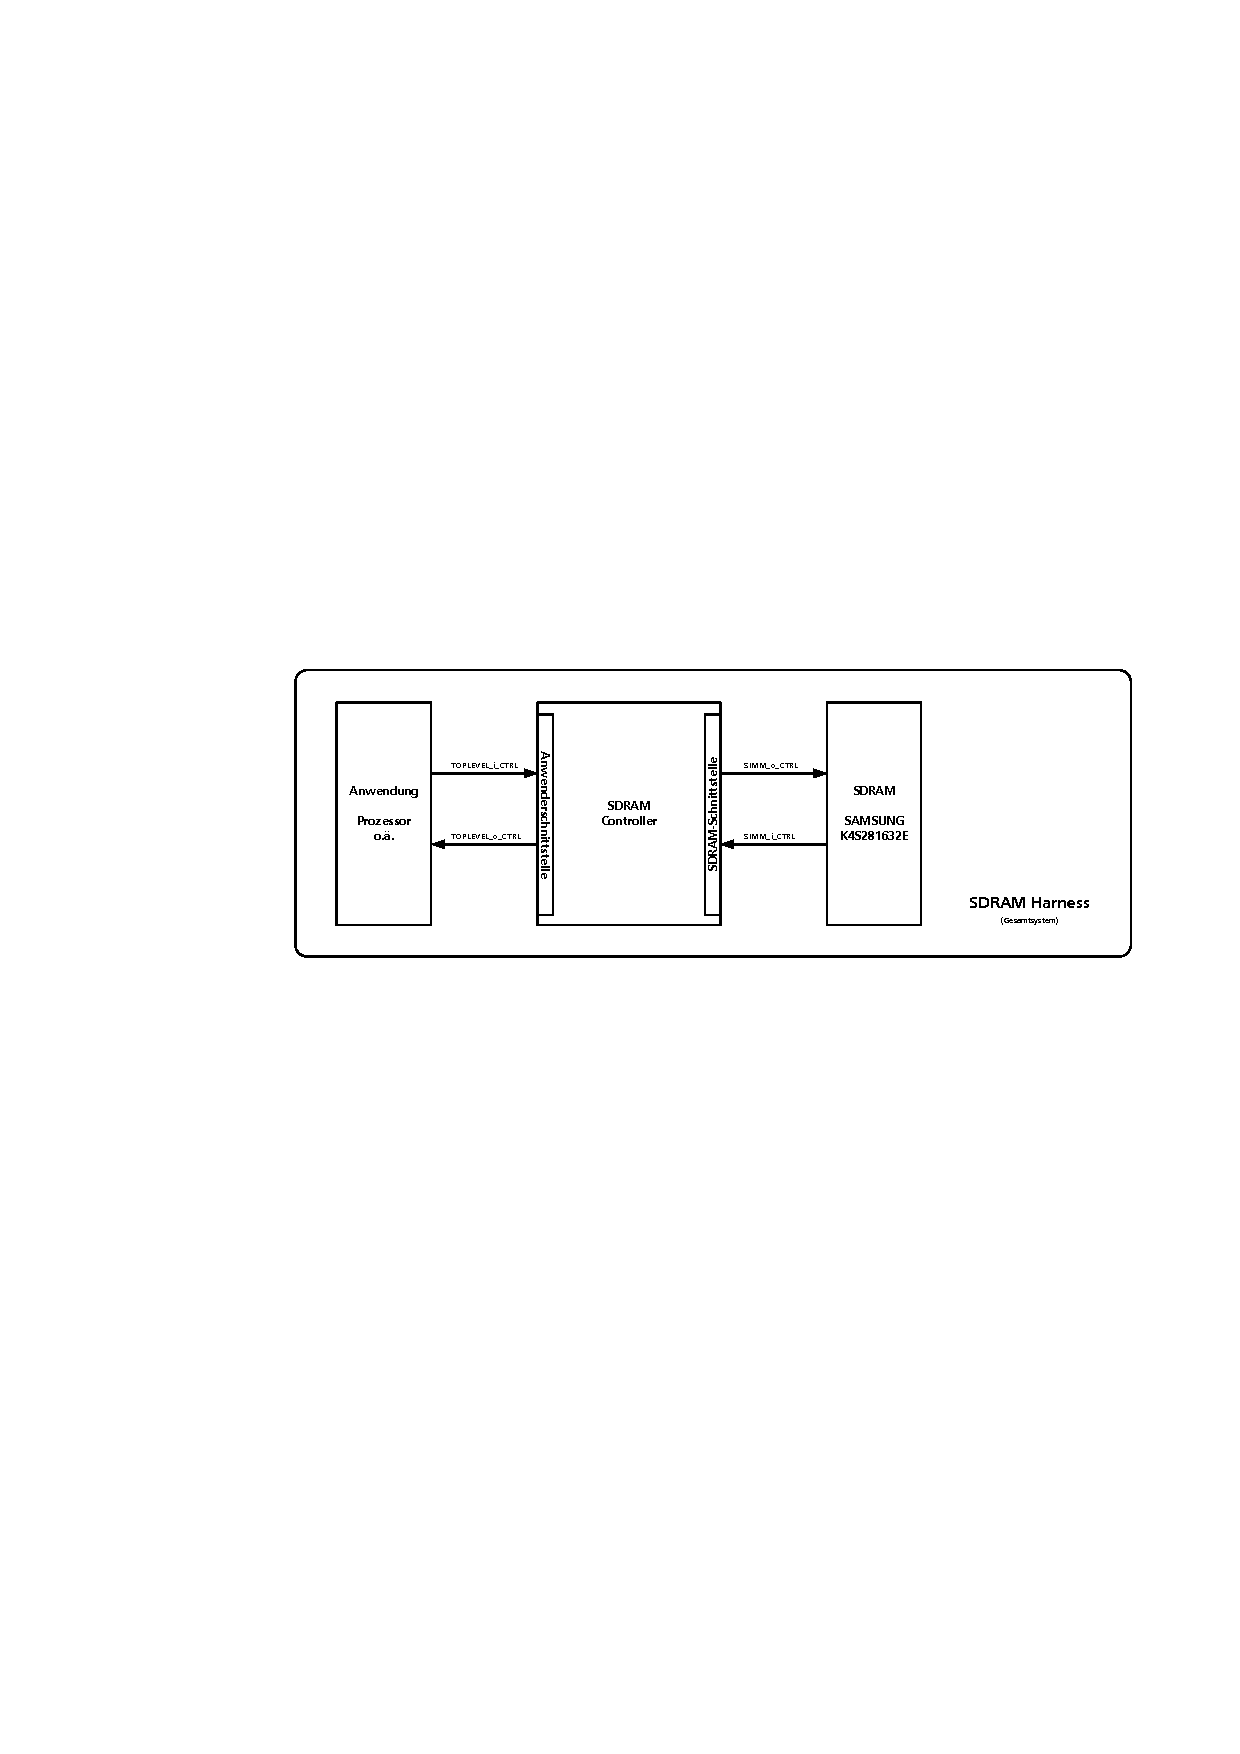
\includegraphics[width=0.66\textwidth]{images/blockschaltbild.pdf}
	\caption{Beispiel: Blockschaltbild \cite{guo}}
	\label{fig:blockschaltbild}
\end{figure}

%\begin{figure}[ht]
%	\centering
%		\includegraphics[width=1.00\textwidth]{images/busy-konflikt.jpg}
%	\caption{Busy-Konflikt im Einzelzugriff.}
%	\label{fig:busy-konflikt}
%\end{figure}

\chapter{Tabellen}
\label{cha:tabellen}

Um eine einfache Tabelle in Latex zu erzeugen, kann man sich zun�chst mit der tabular � 
Umgebung begn�gen. Die Syntax daf�r ist die folgende: \\
 \\
\textbackslash begin \{tabular\}\{cols\} \\
Tabelleneintr�ge \\
\textbackslash end\{tabular\}\\
 \\
Im Argument ``cols'' gibt man f�r jede Spalte, die in der Tabelle stehen soll, die Ausrichtung 
an. Man hat dabei folgende Optionen: 
 
\begin{table}[ht]
\centering
\begin{tabular}{|c|c|}
\hline
l&Linksb�ndig\\
\hline
r&Rechtsb�ndig\\
\hline
c&Zentriert\\
\hline
p\{x cm\}&Parbox der Breite x cm\\
\hline
\end{tabular}

\caption{Tabellenausrichtung}
\label{tab:Ausrichtung}
\end{table}

 
Will man die Spalten durch einen oder mehrere Striche trennen, so f�gt man mittels der 
Tastenkombination AltGr + ``<'' einen senkrechten Strich (|) zwischen (bzw. vor oder nach) 
den Ausrichtungsangaben ein (siehe Beispiele).  
Die Breite der Spalten bestimmt LATEX selbst, es sei denn man gibt eine Parbox an. Die 
Parbox hat den weiteren Vorteil, dass in einer Zelle der Tabelle mehrere Zeilen m�glich sind. 
Weiters kann man mittels Parboxen auch Tabulatoren wie im Word erzeugen. 
 
Die Tabelleneintr�ge werden zeilenweise eingegeben. Dabei erfolgt die Trennung innerhalb 
der Zeile mit ``\&''. Um in die n�chste Zeile zu springen hat man den Befehl ``\textbackslash \textbackslash''. Will man 
auch die Zeilen mittels Strichen trennen, so sind diese mit dem Befehl``\textbackslash hline'' an die 
entsprechende Stelle zu setzen.  
 
Das folgenden Beispiele erl�utern die tabular-Umgebung:  
Mit diesen Kommandos 

\textbackslash begin\{tabular\}\{1p\{10cm\}\}\\
\textbackslash textbf\{tabular\} \& Die Umgebung tabular wird in Latex gew�hlt um einfache Tabellen zu erzeugen\textbackslash\textbackslash\\
\textbackslash textbf\{table\} \& table wird gebraucht um abgesetzte Tabellen zu erzeugen. Die Tabelle kann damit als Gleitobjekt eingef�gt werden\textbackslash\textbackslash\\
\textbackslash textbf\{hline\} \& Mit diesem Befehl kann man mit einem Strich Zeilen trennen\textbackslash\textbackslash\\
\textbackslash textbf\{\textbackslash textbackslash\textbackslash textbackslash\} \& Um auf die n�chste Zeile zu springen\textbackslash\textbackslash\\
\textbackslash end \{tabular\}\textbackslash\textbackslash\\
\\
wird folgende Tabelle erzeugt:\\

\begin{tabular}{lp{10cm}}
\textbf{tabular} & Die Umgebung tabular wird in Latex gew�hlt um einfache Tabellen zu erzeugen\\
\textbf{table}& table wird gebraucht um abgesetzte Tabellen zu erzeugen. Die Tabelle kann damit als Gleitobjekt eingef�gt werden\\
\textbf{hline}& Mit diesem Befehl kann man mit einem Strich Zeilen trennen\\
\textbf{\textbackslash\textbackslash}& Um auf die n�chste Zeile zu springen\\
\end {tabular}\\
\\
\\
Dies ist ein Beispiel, wie man Parboxen zur ``Erzeugung'' von Tabulatoren benutzt werden 
kann. \\
\\
Tabellen, welche mittels der tabular-Umgebung geschrieben werden, werden einfach, wie ein 
gro�er Buchstabe in den Text eingef�gt. Um abgesetzte Tabellen zu erzeugen bedient man 
sich zus�tzlich der table-Umgebung, die die Tabelle als sogenanntes Gleitobjekt einf�gt. Sie 
hat folgende Syntax: 
 
\textbackslash begin\{table\}[Ausrichtung] \\
tabular-Umgebung \\
\textbackslash end\{table\}\\ 
\\
In die eckigen Klammern steht die Ausrichtung. Daf�r hat man folgende Optionen: 

\begin{table}[ht]
\begin{center}
\begin{tabular}{|l|p{8cm}|}
\hline
h&``here''- Tabelle soll an der selben Stelle wie im Quelltext eingerichtet werden\\
\hline
t&``top''- Tabelle wird an den unteren Rand der Seite gestellt\\
\hline
b&``bottom''- Tabelle wird an den unteren Rand der Seite gestellt\\
\hline
p&``page''- Tabelle wird auf einer Gleitobjektseite eingerichtet\\
\hline
\end{tabular}
\end{center}
\caption{table-Ausrichtung }
\label{tab: table Ausrichtung}
\end{table}%

\paragraph{Weiteres Beispiel}
 
Die folgenden Befehle erzeugen eine Tabelle mit Linien: 

\textbackslash begin\{table\}[!h]\\
\textbackslash begin\{center\}\\
\textbackslash begin\{tabular\}\{|l|r|r|r|r|r|\}\\
\textbackslash hline\&\$x\_\{min\}\$\&\$x\_\{0,25\}\$\&\$x\_\{0,5\}\$\&\$x\_\{0,75\}\$\&\$x\_\{max\}\$\textbackslash\textbackslash\\
\textbackslash hline
\textbackslash hline Alter \&14\&19\&20,5\&23\&70\textbackslash\textbackslash\\
\textbackslash hline Semester \&0\&2\&2\&4\&14\textbackslash\textbackslash\\
\textbackslash hline
\textbackslash end\{tabular\}\\


\begin{table}[ht]
\begin{center}
\begin{tabular}{|l|r|r|r|r|r|}
\hline&$x_{min}$&$x_{0,25}$&$x_{0,5}$&$x_{0,75}$&$x_{max}$\\
\hline
\hline Alter &14&19&20,5&23&70\\
\hline Semester &0&2&2&4&14\\
\hline
\end{tabular}
\end{center}
\caption{Verteilung von Alter und Semesteranzahl}
\end{table}


Mehr Informationen �ber Tabellen finden sie \htmladdnormallink{\underline{hier}}{http://www.ifas.jku.at/Portale/Institute/SOWI_Institute/ifas/content/e3413/e3414/files7134/TabelleninLATEX.pdf}.





%% Anhang %%%%%%%%%%%%%%%%%%%%%%%%%%%%%%%%%%%%%%%%%%%%%%%%%%%%%%%%%%%%%%%%
%\appendix
\bibliographystyle{plain}
\clearpage
% \nocite{*}
\bibliography{literaturverzeichnis}


\end{document}
